\section{Results}
\label{sec:results}
Following, we will perform an exploratory analysis of our study results.

\begin{figure}
\centering
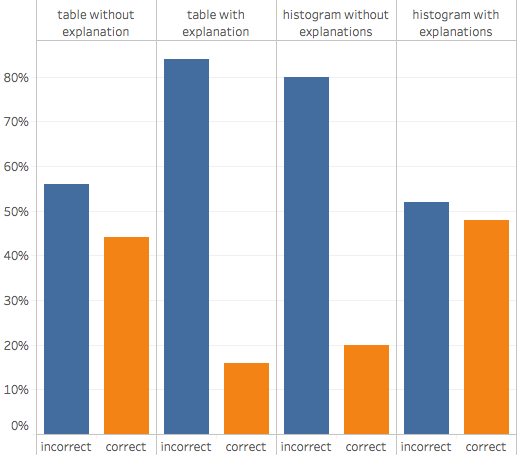
\includegraphics[width=0.5\linewidth]{aggexplain/correctness}
\caption[Comparing whether participants correctly identified the bias.]{
Comparing whether participants correctly identified the bias in the data, determined from plain-text answers. Note, that adding explanations to the table view hurt performance, whereas adding explanations to the histogram view improved performance.
}
\label{figs:correctness}
\end{figure}

For reasons we will explore later, we used the plain-text answers of the participants to determine whether they correctly found the bias in the correct data set.
This is an unambiguous way, since participants were verbose about their findings (if they found something):
``It has higher accuracy so should be more trustworthy than the other one. However some of the results don't make sense to me. Maybe this is just an atypical property market.'';
``It is accurate, yet the predictions do not make much sense. Higher quality houses having a larger amount of low priced houses, percentage-wise? More rooms, area, or stories resulting in lower prices? The logic does not work out.'';
``larger houses are valued lower than others which are smaller''.

% \begin{figure}
% \centering
% 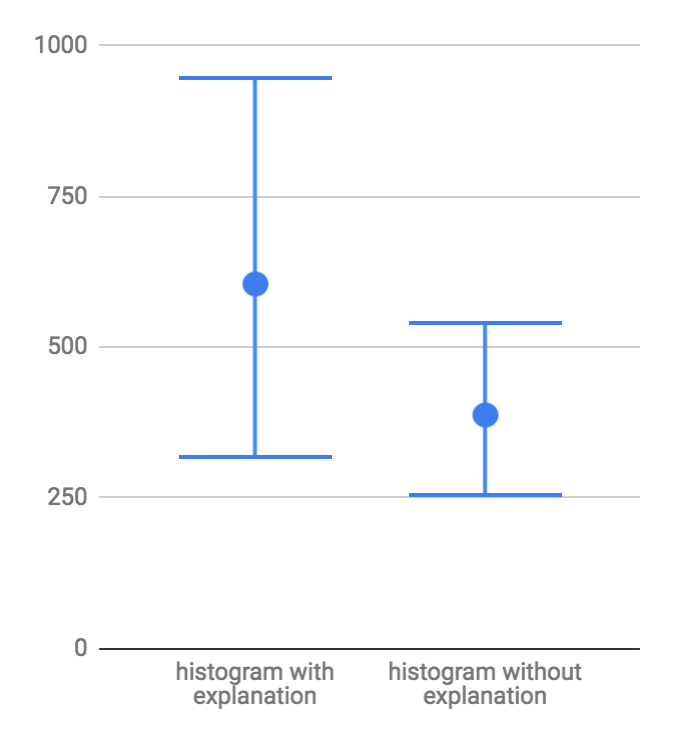
\includegraphics[width=0.4\linewidth]{figs/hist_interaction}
% \caption{
% Interaction with the histogram view measured by counting how many histogram bars were hovered by the mouse.
% The plot shows the bootstrapped mean and confidence interval for each setting.
% }
% \label{figs:hist_interaction}
% \end{figure}

Comparing the correctness across all four conditions can be seen in Figure~\ref{figs:correctness}.
First, we can see a strong improvement in correctness when adding explanations to histograms (p-value Fisher's $0.0359$, $\chi^2$ $0.0366$) or when switching from tables to histograms while having access to explanations (p-value Fisher's $0.0161$, $\chi^2$ $0.0169$).
We hypothesize that explanations are a necessity for histograms to work effectively, since they point out which, of the possibly many, pattern seen in the distributions are meaningful.
% The engagement with the histogram view was also higher when explanations were available (see Figure~\ref{figs:hist_interaction}).

\begin{figure}[t]
\centering
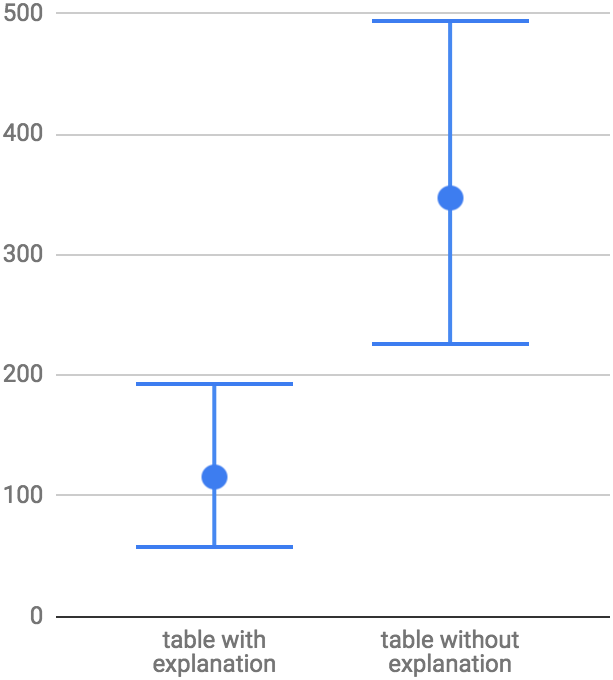
\includegraphics[width=0.25\linewidth]{aggexplain/table_interaction}
\caption[Interactions with the table view.]{
Interactions with the table view measured by counting how many table cells were hovered by the mouse.
The plot shows the bootstrapped mean and confidence interval for each setting.
}
\label{figs:table_interaction}
\end{figure}

However, we see a strong decline in correctness when adding explanations to tables (p-value Fisher's $0.0311$, $\chi^2$ $0.0320$).
At first, we were puzzled at this counter-intuitive result and we double and triple checked that those results were not a simple mix-up in conditions.
We hypothesize that, having explanations at hand in a table, focuses the attention of participants to fewer instances and additionally makes them more confident that they fully understood the model.
This extrapolation from few instances aligns with the findings of Stumpf~\etal~\cite{harmful}, who found that explanations can be harmful in certain circumstances.

\begin{figure}
\centering
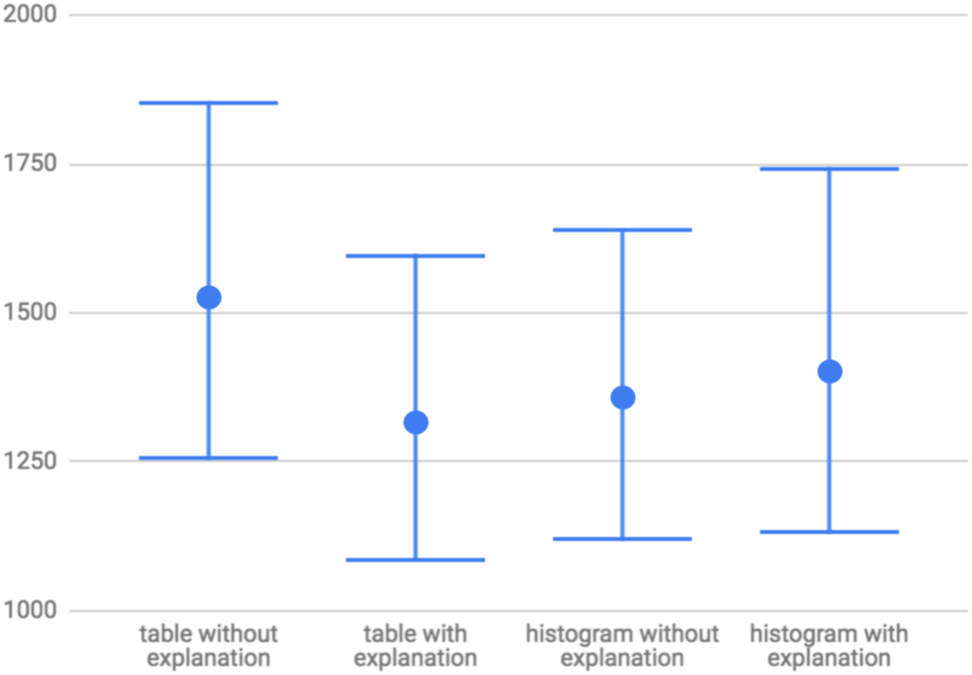
\includegraphics[width=0.4\linewidth]{aggexplain/timing2}
\caption[Overall completion time of the study divided by condition.]{
Overall completion time of the study divided by condition.
The plot shows the bootstrapped mean and confidence interval for each setting.
There is no significant difference between the conditions.
}
\label{figs:timing}
\end{figure}

In order to investigate this hypothesis further, we can look at the number of interactions of the participants performing the tasks.
We can see in Figure~\ref{figs:table_interaction} that participants engaged with the table view significantly more when no explanations were present.
This might be an example of Hullman~\etal~\cite{6064986}, which states that information visualization might benefit from visual difficulties, as is the case with a table without any further help from the interface about what to look at, since people are forced to interact more with the visualization.

% \begin{figure}
% \centering
% 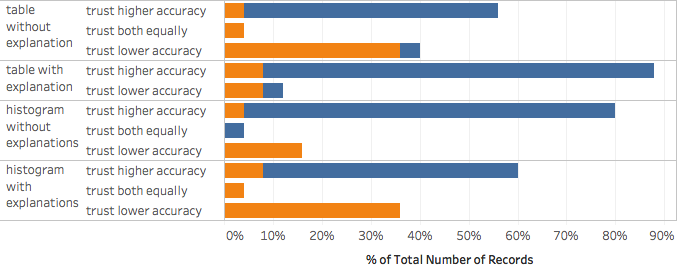
\includegraphics[width=0.75\linewidth]{figs/trust}
% \caption{
% The participants' answer to whether they trust the model with higher accuracy, lower accuracy, or both equally. The orange colored part indicates the proportion of participants that correctly found the bias in the data.
% Note, that some participants valued accuracy more than semantically correct data.
% }
% \label{figs:trust}
% \end{figure}

Despite that, we found no significant difference in the time participants took to complete the study, as can be seen in Figure~\ref{figs:timing}.
% Additionally, Figure~\ref{figs:timing} also shows that participants spent less time on the histogram view with explanations than on the table view without explanations.
Even though the histogram view with explanations and the table view without explanations do not have a significant timing difference, we hypothesize that an aggregated representation of the model is a more effective method for finding biases.
This hypothesis is rooted in both conditions performing equally well and histograms being a more scalable data representation than tables, since due to their independence from the magnitude of the data.

As mentioned earlier, we chose the participants' written answers to determine whether the participant correctly identified the bias in the data.
Even though participants correctly identified the flaw in the data, it sometimes was not enough to convince them that the corresponding model cannot be trusted as much:
``If the data says it's true, then it's true I suppose and it's more trustworthy than my common sense.'';
``I feel like the results of [the biased model] where strange even though they where correct according to the dataset.'' (sic);
``I'm drawn to trusting the model which was more accurate even though it didn't entirely make sense to me.''.

$25\%$ of people who correctly identified the bias still opted to trust the biased model more, due to the higher reported accuracy of the model.
A further $8\%$ who identified the bias trusted both models equally.
Again, this aligns with the findings of Stumpf~\etal~\cite{harmful} that trust in the machine learning model may \emph{override} people's initial intuition about its performance.

% We categorized the written answers of the participants and noted when participants correctly detected the flaw in the biased data set (see Figure~\ref{figs:correctness}).
% Looking at the figure we can see a significant\todo{compute as well} improvement in correctly detected biases when changing either from the table view to the histogram view or from the having no explanations to having explanations.
% However, the condition of the table view without explanations has the highest rate of correct answers.
% Looking at the overall completion time (Figure~\ref{figs:timing}) we can see that participants without any help in form of aggregation or explanations spent more time analyzing the data set (Note, that the figure does not include extreme outliers at maximum 3 hours).
% This more thorough explanation enables the participants to find the bias in the data set even under non helpful conditions.
% In terms of trust (see Figure~\ref{figs:trust}) participants of the histogram view with explanations trust the correct model significantly\todo{compute} more than in the conditions with either only the histogram view or the table view with explanations.
% This is mostly in agreement with the ability to correctly identify the bias.
% However, some participants dismiss the unbiased model in favor of the higher accuracy of the biased model under all conditions: ``If the data says it's true, then it's true I suppose and it's more trustworthy than my common sense.''; ``I feel like the results of model 2 where strange even though they where correct according to the dataset.''; ``I'm drawn to trusting the model which was more accurate even though it didn't entirely make sense to me.''
% This might be partially rooted in the participants not feeling ``expert'' enough but stemmed mostly from regarding accuracy higher than the bias in the data.
% This aligns with the findings of Stumpf~\etal~\cite{harmful}.
